\documentclass[11pt]{beamer}

\graphicspath{{Images/}{./}}
\usepackage{booktabs}
\usetheme{Madrid}

\usefonttheme{default} % Typeset using the default sans serif font

\usepackage{palatino} % Use the Palatino font for serif text

\usepackage[default]{opensans} % Use the Open Sans font for sans serif text
\usepackage[makeroom]{cancel}
\usepackage{makecell}
\useinnertheme{circles}
\usepackage{colortbl}
\newcommand{\light}[1]{\textcolor{gray}{#1}}
\usepackage{xcolor}
\DeclareMathOperator*{\mean}{mean}
\title[DSA Scale Uncertainty]{Addressing Scale Uncertainty in Differential Set Analysis}

\author[Kyle McGovern]{Kyle McGovern}

\institute[Penn State]{The Pennsylvania State University \\ \smallskip \textit{kvm6065@psu.edu}} 

\date[\today]{GLBIO 2024 \\ \today}

%----------------------------------------------------------------------------------------

\begin{document}

%----------------------------------------------------------------------------------------
%	TITLE SLIDE
%----------------------------------------------------------------------------------------

\begin{frame}
	\titlepage
\end{frame}

\begin{frame}
  \begin{center}
    What scientific question are we asking of our sequence count data?
  \end{center}
\end{frame}

\begin{frame}
  \frametitle{What is Our Scientific Question?}

  \begin{center}
    \underline{\textbf{Differential Expression/Abundance (DE/DA) Analyses}}
  \end{center}
  
  \begin{itemize}
    \item Is the TNF\(\alpha\) gene upregulated in tumor tissue?

    \begin{center}
      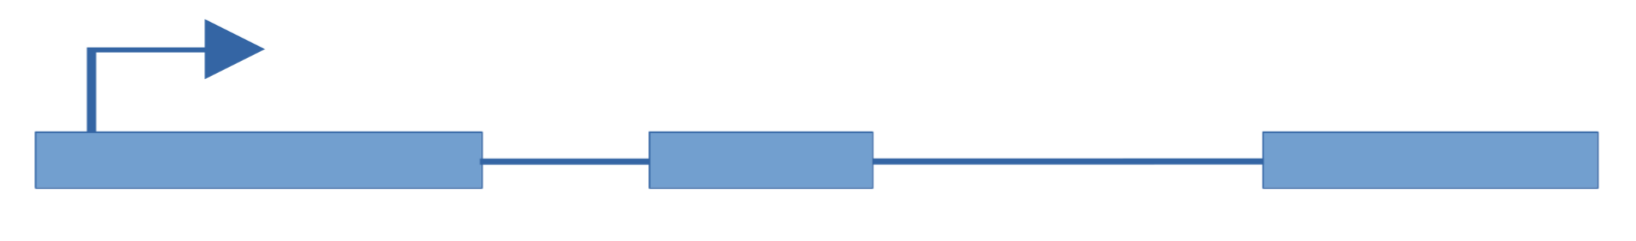
\includegraphics[scale=0.17]{/home/hh/data/output/single_gene.png}
    \end{center}


    \item Is the \textit{S. pyogenes} bacetrium killed by an antibiotic?
        
     \begin{center}
      
\includegraphics[scale=0.04]{/home/hh/data/output/single_microbe.png}
    \end{center}

      
  \end{itemize}
  
  \vspace{10px}
  \underline{Methods for DE/DA}: ALDEx2, DESeq2, etc.
  
\end{frame}

\begin{frame}
   \begin{center}
    But what if we have questions of higher level biological processes (e.g., gene pathways)?
   \end{center}

   \begin{center}
      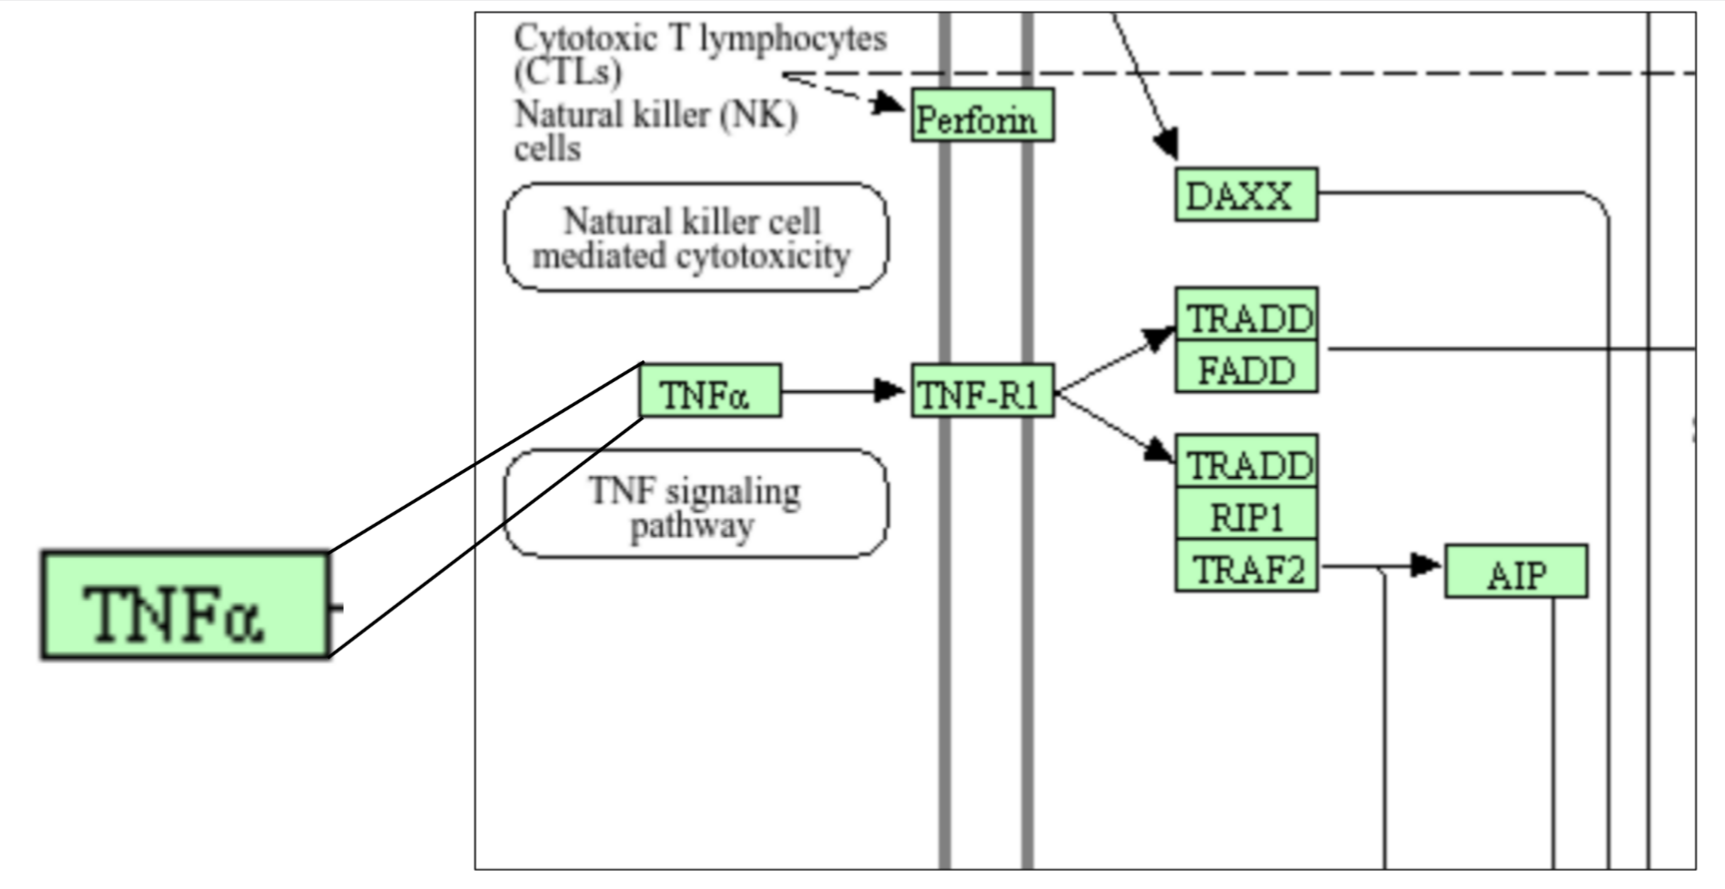
\includegraphics[scale=0.18]{/home/hh/data/output/pathway_z.png}
    \end{center}

\end{frame}

\begin{frame}
  \frametitle{What is Our Scientific Question?}
  
  \begin{center}
    \underline{\textbf{Differential Set Analysis (DSA)}}
  \end{center}

  \begin{itemize}
    \item Is the \textbf{Apoptosis pathway} upregulated in tumor tissue?
    \item Are \textbf{anaerobic bacetria} killed by an antibiotic?
  \end{itemize}

  \vspace{100px}
  \underline{Methods for DSA}: GSEA, CAMERA, etc.
  
\end{frame}

\begin{frame}
  \frametitle{Review of the Problem of Scale}

  \begin{block}{Example Experiment}
    Conisder 16S rRNA sequencing of fecal samples to measure \(D\) taxa in the colons of \(N\) individuals with and without IBS.
  \end{block}

  \pause

  \begin{alertblock}{Problem of Scale}
    \begin{itemize}
      \item We want to analyze absolute abundances (\(W\))
      \item Absolute abundances are only known if the composition (\(W^\parallel\)) and scale (\(W^\perp\)) are known
      \item Sequence count data only measure the composition
    \end{itemize}
  \end{alertblock}
  
  \begin{align*}
    \underbrace{W_{dn}}_{\substack{\text{Absolute Abundance} \\ \text{Taxa d, Patient n} \\ \text{\textcolor{red}{(Unmeasured)}}}} = \underbrace{W^\parallel_{dn}}_{\substack{\text{Composition} \\ \text{Taxa d, Patient n} \\ \text{\textcolor{green}{(Measured)}}}} \times \underbrace{W^\perp_n}_{\substack{\text{Scale} \\ \text{(e.g., total \# of microbes in} \\ \text{patient n's colon)} \\ \text{\textcolor{red}{(Unmeasured)}}}}
  \end{align*}
\end{frame}

\begin{frame}
  \frametitle{DE/DA Estimation of LFCs}

  \begin{block}{Example Experiment}
        Conisder 16S rRNA sequencing of fecal samples to measure \(D\) taxa in the colons of \(N\) individuals with and without IBS.
  \end{block}

  \vspace{15px}
  
  The Log Fold Change (LFC) in absolute abundance of taxa \(d\) is
  \begin{align*}
    \theta_d = \mean_{n \in \text{IBS}}(\log W_{dn}) - \mean_{n \in \text{Healthy}}(\log W_{dn} )
  \end{align*}

\end{frame}

\begin{frame}
  \frametitle{DE/DA Estimation of LFCs}
  
  The Log Fold Change (LFC) in absolute abundance of taxa \(d\) is
  \begin{align*}
    \theta_d = \mean_{n \in \text{IBS}}(\log W_{dn}) - \mean_{n \in \text{Healthy}}(\log W_{dn} )
  \end{align*}

  Using the relationship \(W_{dn} = W^\parallel_{dn} \times W^\perp_n\):
  {\small
  \begin{align*}
    \small
    \theta_{d} &= \mean_{n \in \text{IBS}}(\log W_{dn})-\mean_{n \in \text{Healthy}}(\log W_{dn}) \\
&= \underbrace{\left[\mean_{n \in \text{IBS}}(\log W^{\parallel}_{dn}) - \mean_{n \in \text{Healthy}}(\log
    W^{\parallel}_{dn})\right]}_{\theta^\parallel_d}+\underbrace{\left[\mean_{n \in \text{IBS}}(\log W^{\perp}_{n}) - \mean_{n \in \text{Healthy}}(\log W^{\perp}_{n})\right]}_{\theta^\perp} \label{eq:diff-analysis-2} \\
                         &= \theta_{d}^{\parallel}+\theta^\perp. \nonumber
  \end{align*}
  }%
\end{frame}

\begin{frame}
  \frametitle{DE/DA Estimation of LFCs}

  The LFC can be decomposed into compositional and scale terms as 
  \begin{align*}
    \underbrace{\theta_d}_{\text{LFC (Microbe d)}} = \underbrace{\theta_d^\parallel}_{\substack{\text{LFC in} \\ \text{composition (Microbe d)}}} + \underbrace{\theta^\perp}_{\substack{\text{LFC in} \\ \text{scale}}}
  \end{align*}

  \pause

  Using vector notation for all genes/microbes:
  \begin{align*}
    \begin{bmatrix} \theta_1 \\ \vdots \\ \theta_D \end{bmatrix} &= \begin{bmatrix} \theta^\parallel_1 \\ \vdots \\ \theta^\parallel_D \end{bmatrix} + \begin{bmatrix} 1 \\ \vdots \\ 1 \end{bmatrix} \theta^\perp \\
    \theta &= \theta^\parallel + \pmb{1}\theta^\perp
  \end{align*}
\end{frame}


\begin{frame}
  \frametitle{DE/DA Estimation of LFCs}

  \pause

  Methods like DESeq2, ALDEx2, etc. are functions of the sequence count data \(Y\):
  \begin{align*}
    f(Y) &= \underbrace{\hat{\theta}}_{\text{Estimated LFC}} \\
         &= \underbrace{\hat{\theta}^\parallel}_{\substack{\text{Estimated LFC} \\ \text{in Composition}}} + \underbrace{\pmb{1}\hat{\theta}^\perp}_{\text{Scale Assumption}}
  \end{align*}

  \pause

  \begin{exampleblock}{Scale Assumption \(\hat{\theta}^\perp\)}
    \begin{itemize}
      \item Remember \(\theta^\perp\) is unmeasured
      \item Methods like ALDEx2, etc. estimate \(\theta^\perp\) through \textbf{normalization}
      \item Normalizations imply assumptions about the unmeasured \(\theta^\perp\)
    \end{itemize}
  \end{exampleblock}
\end{frame}

\begin{frame}
  \frametitle{Scale Assumptions and Normalization}

  Scale assumptions \(\hat{\theta}^\perp\) are made through noramlization:
  \begin{itemize}
    \item Total Sum Scaling (TSS) Normalization assumes \(W^\perp_n=1\), implying
      \begin{align*}
        \hat{\theta}^\perp = 0
      \end{align*}
    \item Centered Log Ratio assumes \(W^\perp_n=1/\text{gm}(W^\parallel_n)\), implying
      \begin{align*}
        \hat{\theta}^\perp = -\mean(\theta^\parallel)
      \end{align*}
  \end{itemize} 
\end{frame}

\begin{frame}
  \frametitle{Errors in Scale Assumptions and LFCs}

  \begin{itemize}
  \item Scale Assumption Error:  
  \begin{align*}
    \underbrace{\theta^\perp}_{\text{True LFC in Scale}} = \underbrace{\hat{\theta}^\perp}_{\text{Scale Assumption}} + \underbrace{\epsilon^\perp}_{\text{Scale Assumption Error}}
  \end{align*}

  \pause
  
  \item Ignoring compositional error, i.e., assuming:
    \begin{align*}
      \theta^\parallel = \hat{\theta}^\parallel
    \end{align*}

    \pause

  \item The relationship between the LFC and scale error is then
    \begin{align*}
      \underbrace{\theta}_{\text{True LFC}} &= \hat{\theta}^\parallel + \pmb{1}\hat{\theta}^\perp + \pmb{1}\epsilon^\perp \\
                                        &= \underbrace{\hat{\theta}}_{\text{Estimated LFC}} + \underbrace{\pmb{1}\epsilon^\perp}_{\text{Scale Assumption Error}}
    \end{align*}
  \end{itemize}
\end{frame}

\begin{frame}
  \frametitle{LFC Sensitivity Analysis}

    \begin{align*}
      \underbrace{\theta}_{\text{True LFC}} &= \underbrace{\hat{\theta}}_{\text{Estimated LFC}} + \underbrace{\epsilon^\perp}_{\text{Scale Assumption Error}}
    \end{align*}

    \vspace{15px}
    \begin{center}
    \begin{block}{LFC Sensitivity Analysis}
      How do the results of a method as a function of error \(\epsilon^\perp\)?
    \end{block}  
    \end{center}
\end{frame}

\begin{frame}
  \frametitle{For DE/DA LFC Sensitivity Analysis is Not Interesting}

  [Insert image from Justin's slides]
\end{frame}

\begin{frame}
  \begin{center}
    But is LFC Sensitivity Analysis for DSA interesting?
  \end{center}
\end{frame}

\begin{frame}
  \frametitle{DSA Target of Inference}

  Let \(S=\{s_1,\dots,s_K\}\) where \(s_k \in  \{1,\dots,D\}\) be a set of genes or microbes.

  \vspace{15px}

  The goal of DSA is to infer \(\phi_S\) where
  \begin{align*}
    \phi_S = \begin{cases}
      1 & \text{If } S \text{ is enriched} \\
      -1 & \text{If } S \text{ is depleted} \\
      0 & \text{If } S \text{ is neither enriched/depleted}
    \end{cases}
  \end{align*}

  \vspace{15px}

  The Gene Set Enrichment Analysis (GSEA) method is a popular tool for estimating \(\phi_S\)
  
\end{frame}

\begin{frame}
  \frametitle{GSEA with Gene Label Permutations}

  GSEA test statistic calculation:
  \begin{enumerate}
    \item Estimate LFCs \(\hat{\theta}=f(Y)\) and rank in descending order
    \item Calculate a \textbf{weighted} running sum iterating down ranked LFCs
      \begin{itemize}
        \item Genes in \(S\) increase running sum by an amount proportional to the LFC
        \item Genes not in \(S\) decrease running sum by constant amount
      \end{itemize}
    \item Enrichment Score is supremum of running sum
  \end{enumerate}
     \begin{columns}
     \begin{column}{0.5\textwidth}
      \begin{center}
        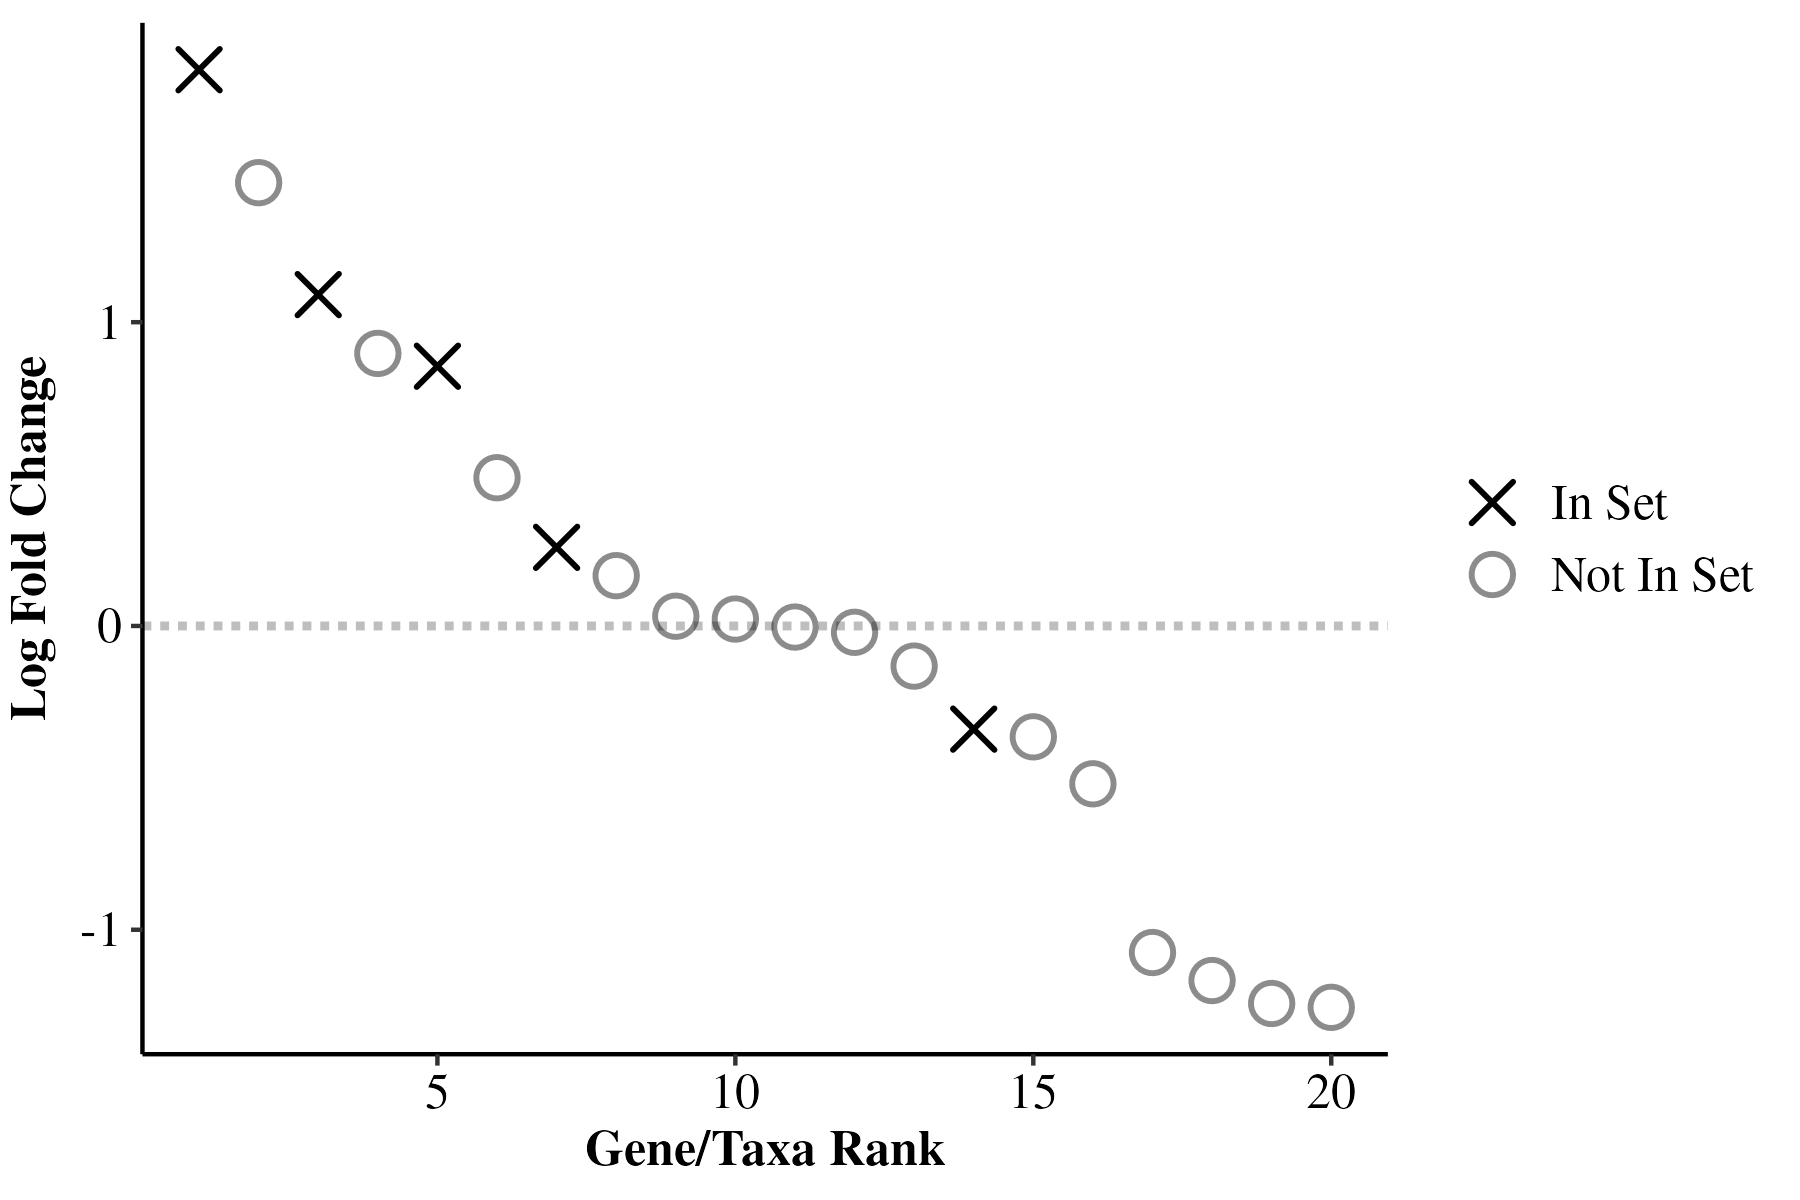
\includegraphics[scale=0.41]{/home/hh/data/output/lfcs_1.png}
      \end{center}
    \end{column}
    \vrule{}
    \begin{column}{0.5\textwidth}  %%<--- here
      \begin{center}
        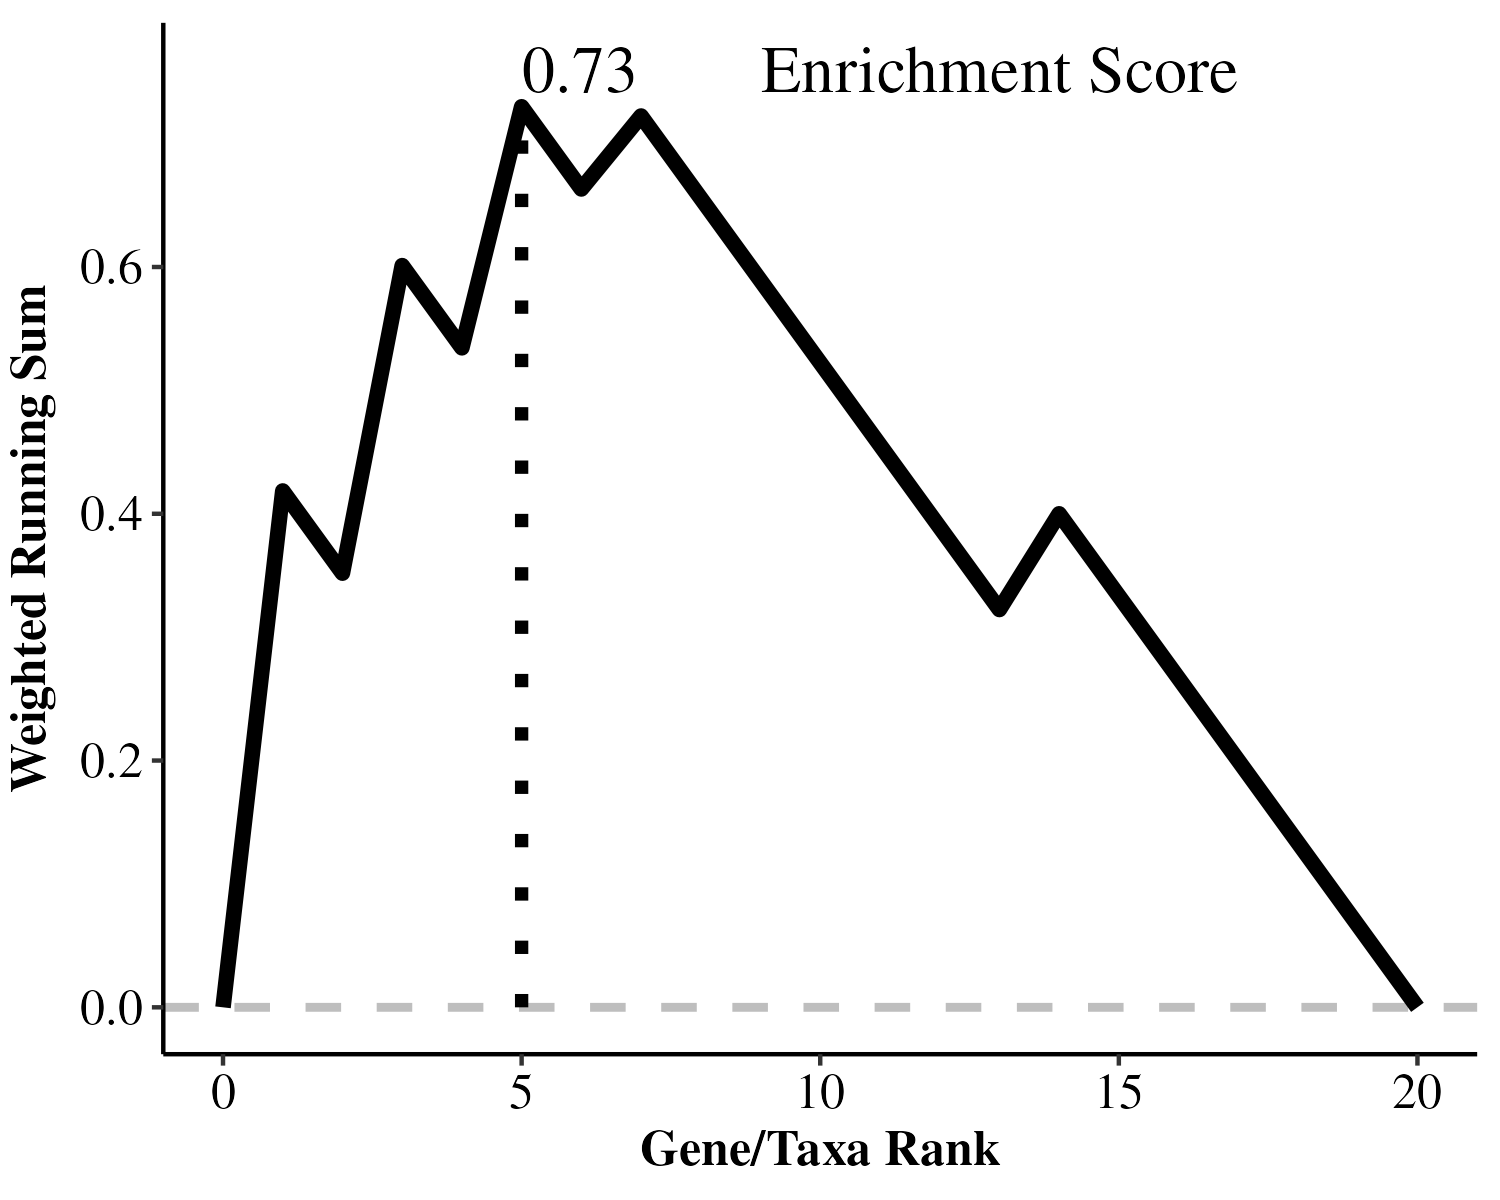
\includegraphics[scale=0.41]{/home/hh/data/output/lfcs_2.png}
      \end{center}
    \end{column}
   \end{columns}
\end{frame}

\begin{frame}
  \frametitle{GSEA with Gene Label Permutations}

  Permutation Statistical Test:
  \begin{enumerate}
    \item Calculate Enrichment Score (ES) for Gene Set \(S\)
    \item Permute gene set labels \(Q\) times, compute null ESs
    \item p-value: \(\# (\text{ES} > \text{Permuted ES}) / Q\)
  \end{enumerate}
  \begin{center}
    \begin{tabular}{| c | c | c | c | c | c | c | c | c | c |}
      \hline
      \makecell{Gene \\Name} & RB1 & IL2 & APP & AR & HTT & IL6 & B2M & RGN & CAT \\
      \hline
      Set \(S\) & X & & X & X & X & & & & \\
      \hline
      \hline
      Perm 1 & & X & X & & & & X & X & \\
      \hline
      Perm 2 & X & & & & & X & X & X & \\
      \hline
      \dots & & & & & & & & & \\
      \hline
      Perm Q & X & & & X & & & X & & X \\
      \hline
    \end{tabular}
  \end{center}
\end{frame}

\begin{frame}
  \frametitle{GSEA and LFC Sensitivity Analysis}

  The GSEA method can be represented mathematically as
  \begin{align*}
    \phi_S = u(\theta)
  \end{align*}

  \pause

  Plugging in
  \begin{align*}
    \underbrace{\theta}_{\text{True LFC}} &= \underbrace{\hat{\theta}}_{\text{Estimated LFC}} + \underbrace{\pmb{1}\epsilon^\perp}_{\text{Scale Assumption Error}}
  \end{align*}

  \pause

  We get
  \begin{align*}
    \phi_S = u(\hat{\theta}+\pmb{1}\epsilon^\perp)
  \end{align*}

  \textbf{How does \(\phi_S\) change with scale assumption error \(\epsilon^\perp\)?}
\end{frame}

\begin{frame}
  \frametitle{GSEA LFC Sensitivity Analysis Simulation Results}

  \begin{center}
    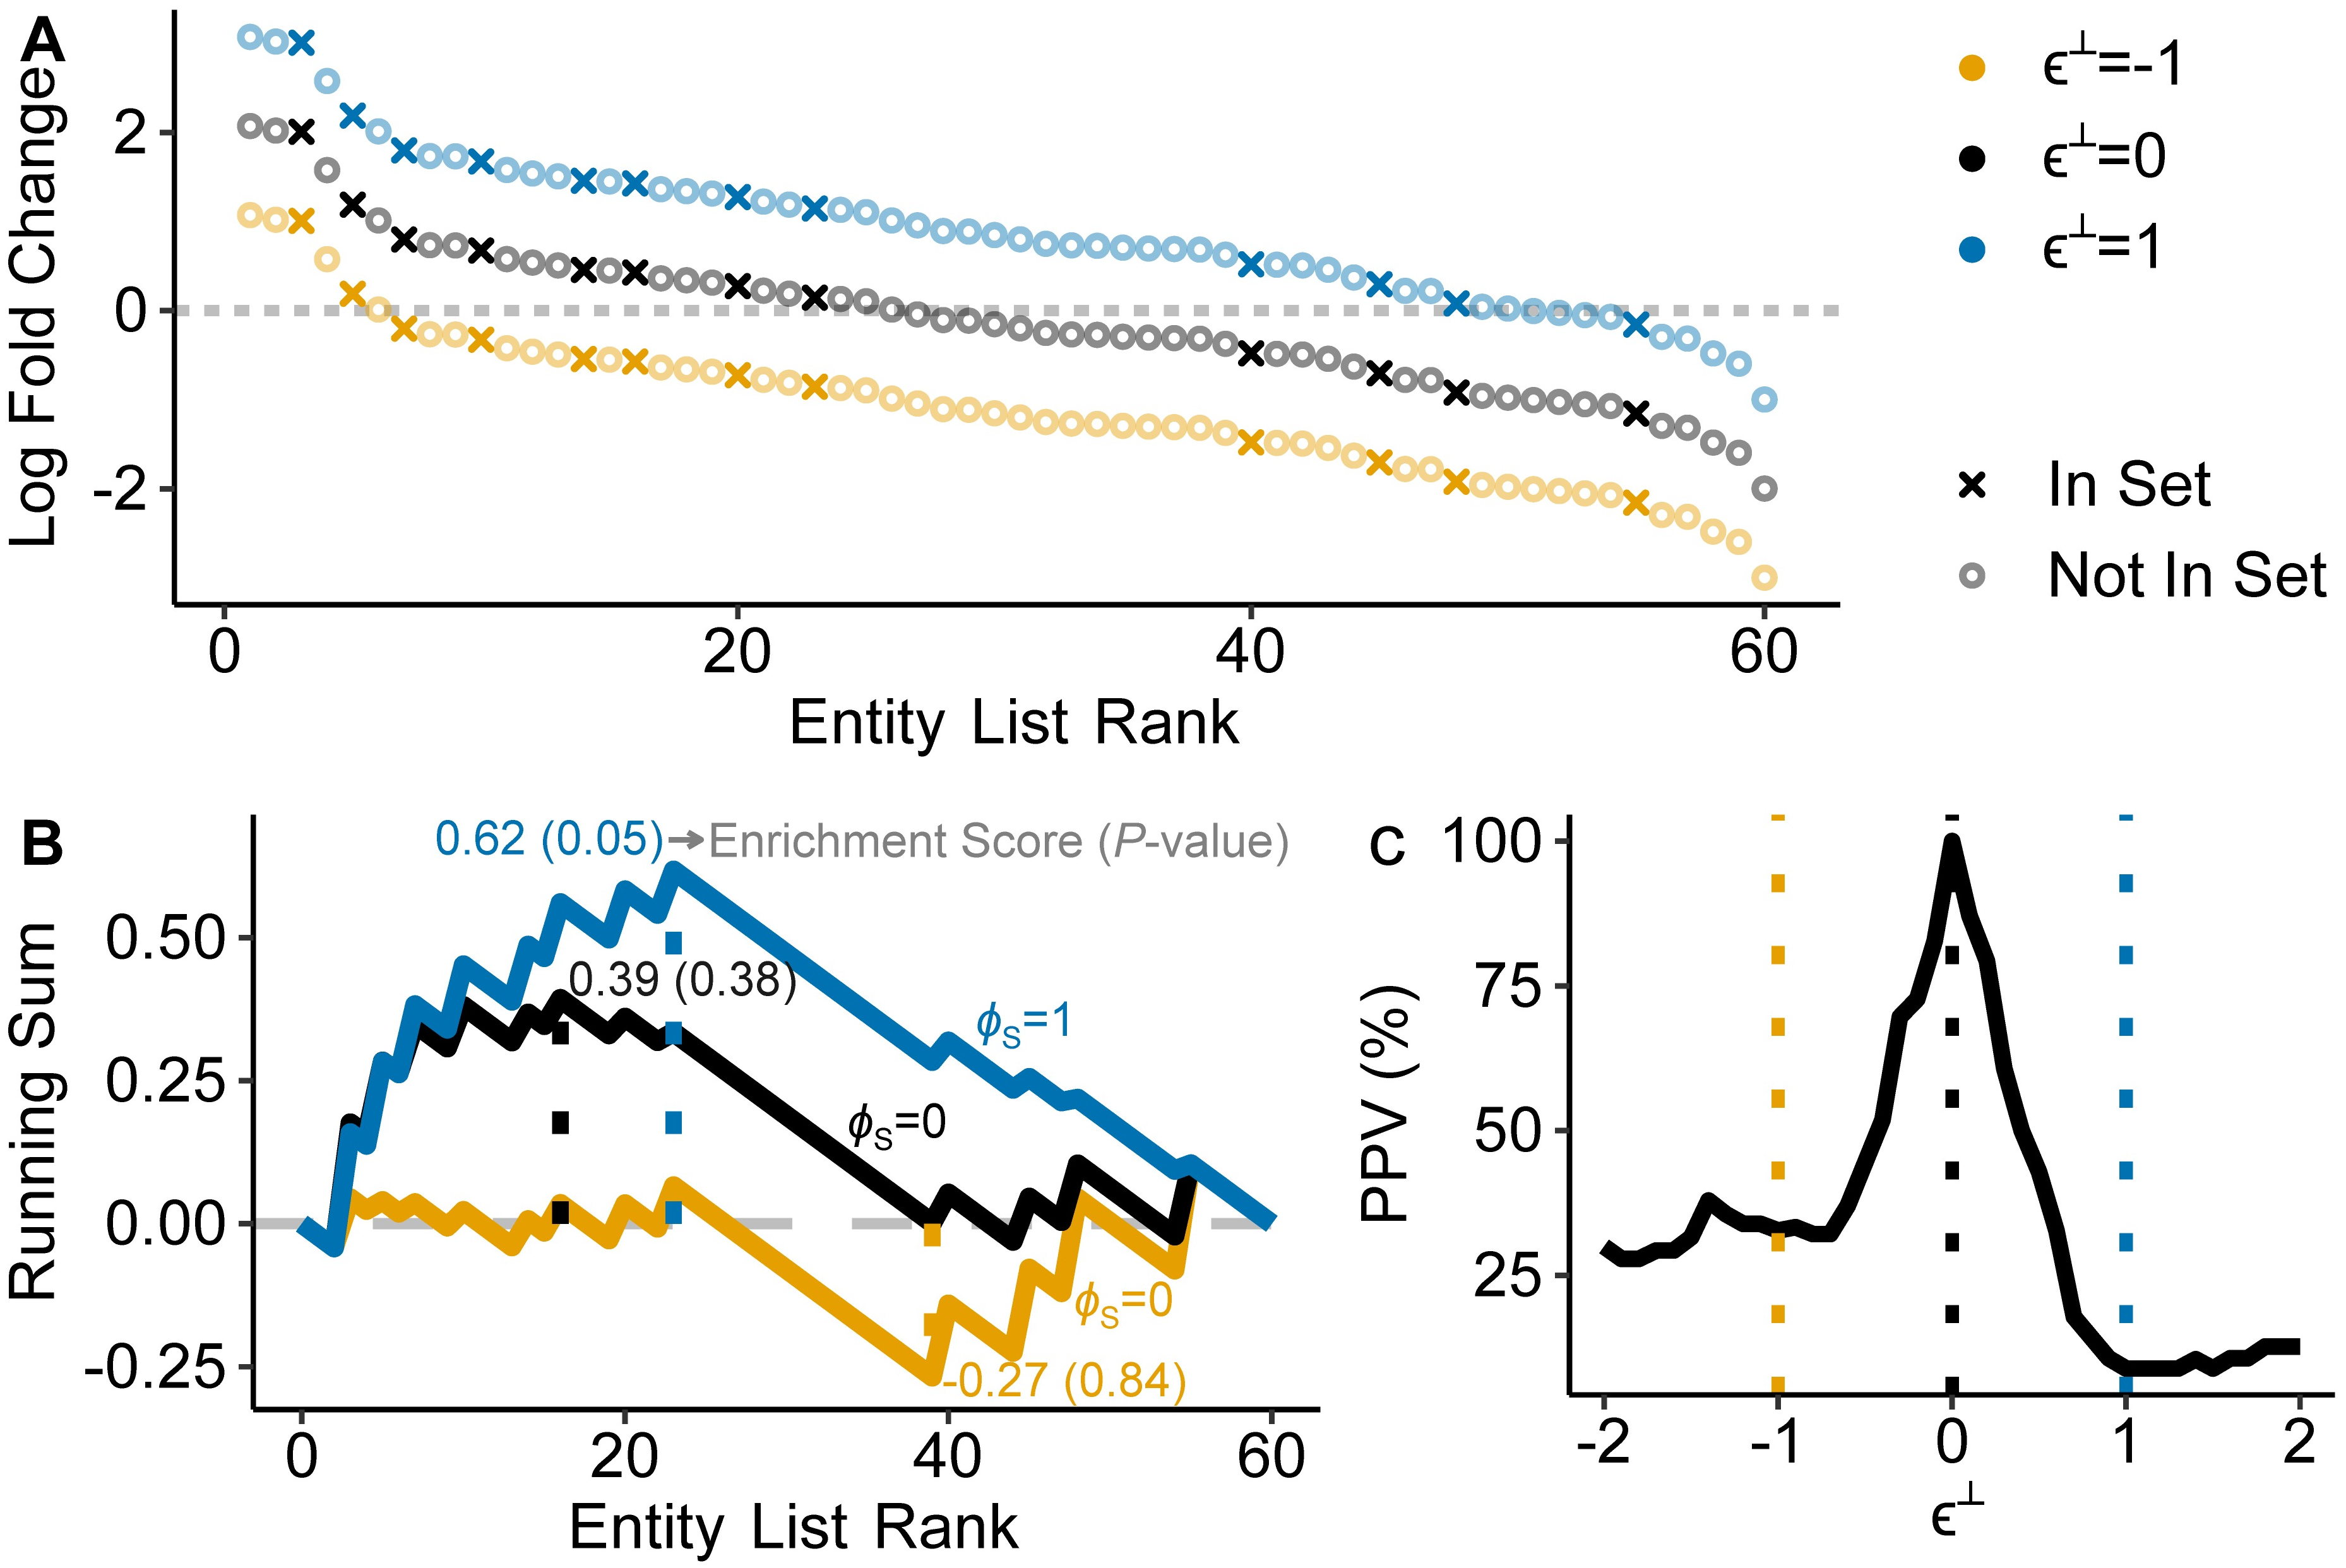
\includegraphics[scale=0.7]{/home/hh/data/output/first_fig.png}
  \end{center}
\end{frame}

\begin{frame}
  \frametitle{GSEA LFC Sensitivity Analysis Real Data Results}

  \begin{center}
    
\includegraphics[scale=0.25]{/home/hh/data/output/paper_image.png}
  \end{center}
  
\end{frame}

\begin{frame}
   \frametitle{Healthy vs. NAT Tissue Research Question}
   \begin{columns}
     \begin{column}{0.5\textwidth}
      \begin{center}
        \underline{Healthy}
        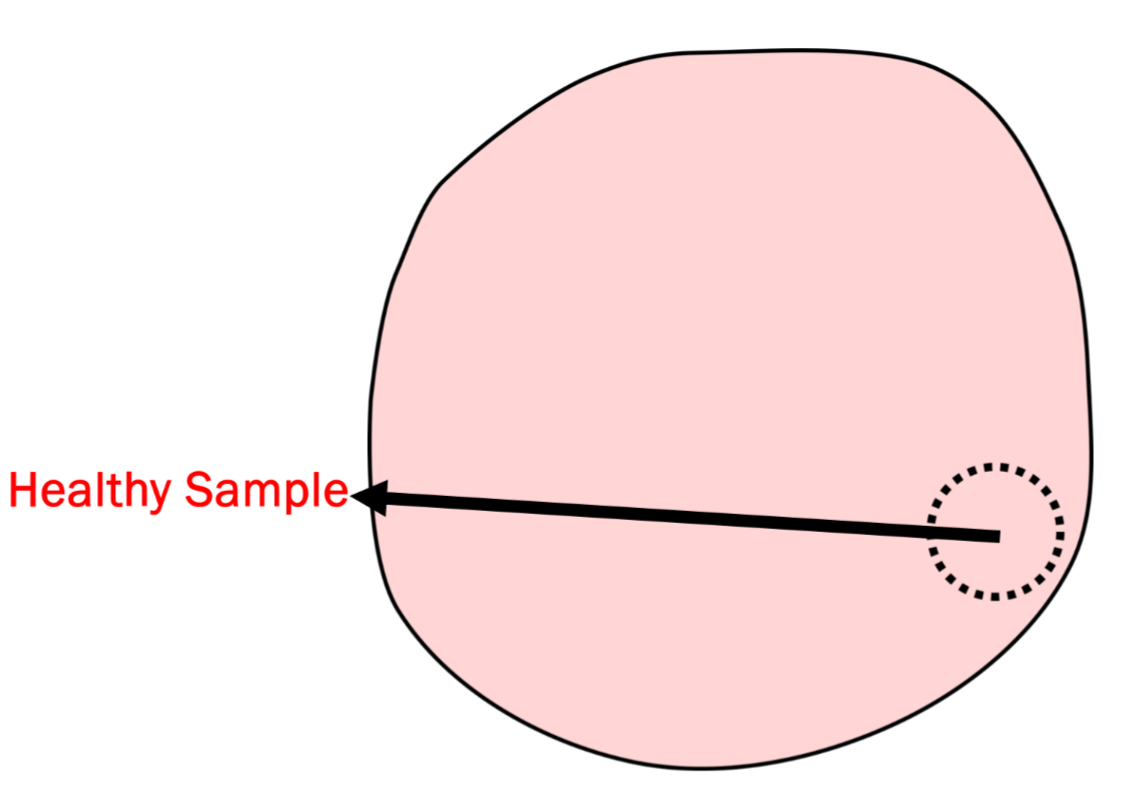
\includegraphics[scale=0.16]{/home/hh/data/output/healthy.png}
      \end{center}
    \end{column}
    \vrule{}
    \begin{column}{0.5\textwidth}  %%<--- here
      \begin{center}
        \underline{Normal-Adjacent-to-Tumor (NAT)}
        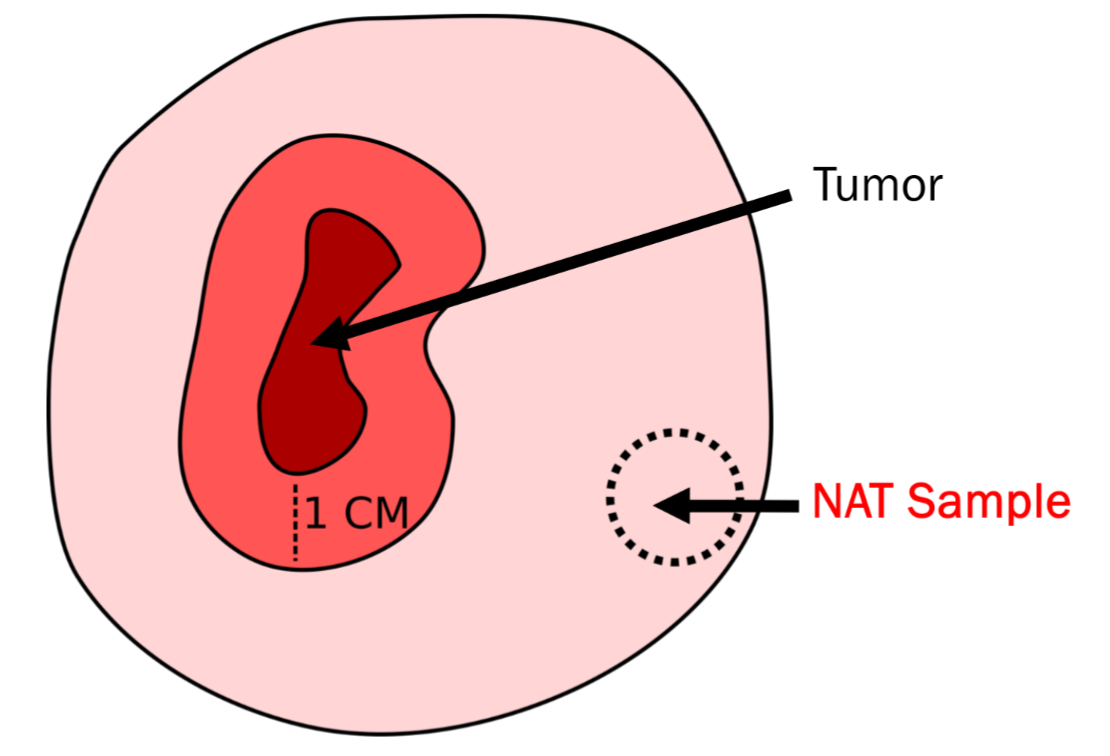
\includegraphics[scale=0.16]{/home/hh/data/output/nat.png}
      \end{center}
    \end{column}
   \end{columns}
   \begin{exampleblock}{Research Question}
     Is NAT tissue an appropriate proxy for healthy tissue in cancer research?
   \end{exampleblock}
\end{frame}

\begin{frame}
  \frametitle{Aran et al. GSEA Results}
  \begin{center}
    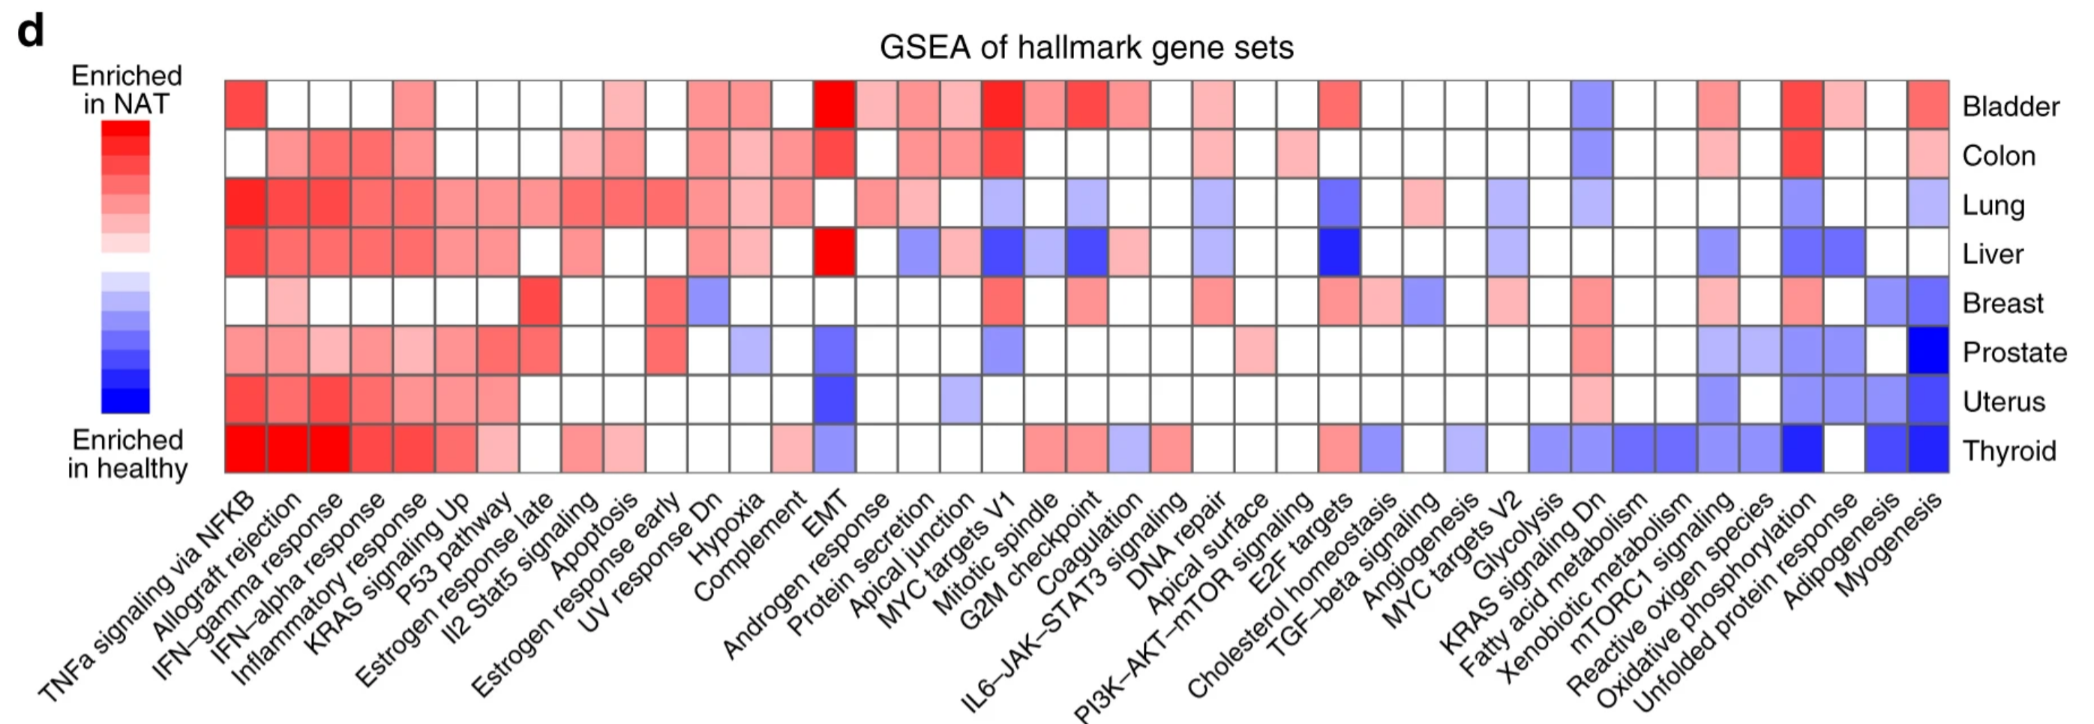
\includegraphics[scale=0.17]{/home/hh/data/output/aran_res.png}
  \end{center}
\end{frame}

\begin{frame}
  \frametitle{NAT vs. Healthy Thyroid Tissue}
  
  Results using the fast GSEA (fgsea) package:
    \begin{center}
    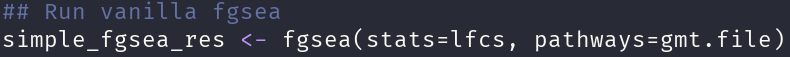
\includegraphics[scale=0.37]{/home/hh/data/output/vanilla_fgsea.png}
  \end{center}
  \begin{columns}
    \begin{column}{0.5\textwidth}
      \begin{center}
        \underline{Myogenesis}
        
        \begin{tabular}{ |c|c| } 
        \hline
        adj. p-val & \textbf{9e-9} \\
        \hline
        NES & -2.1 \\
        \hline
        \end{tabular}
      \end{center}
    \end{column}
    \vrule{}
    \begin{column}{0.5\textwidth}  %%<--- here
      \begin{center}
        \underline{Inflamatory Response}
        
        \begin{tabular}{ |c|c| } 
        \hline
        adj. p-val & \textbf{3e-3} \\
        \hline
        NES & 1.5 \\
        \hline
        \end{tabular}
      \end{center}
    \end{column}
  \end{columns}

  \pause

  \vspace{10px}
  Results using fgsea \textbf{LFC Sensitivity Analysis} wrapper:
  \begin{center}
    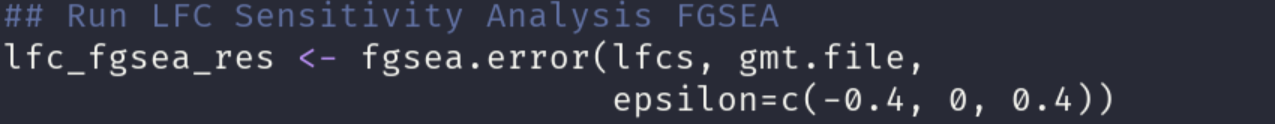
\includegraphics[scale=0.25]{/home/hh/data/output/lfc_sens.png}
  \end{center}
  \begin{columns}
    \begin{column}{0.5\textwidth}
      \begin{center}
        \begin{tabular}{ |c|c|c|c| } 
        \hline
        \(\epsilon^\perp\) & \(-0.4\) & \(0\) & \(0.4\) \\
        \hline
        adj. p-val & \textbf{2e-6} & \textbf{9e-9} & \textbf{2e-9} \\
        \hline
        NES & -1.4 & -2.1 & -2.5 \\
        \hline
        \end{tabular}
      \end{center}
    \end{column}
    \vrule{}
    \begin{column}{0.5\textwidth}  %%<--- here
      \begin{center}
        \begin{tabular}{ |c|c|c|c| } 
        \hline
        \(\epsilon^\perp\) & \(-0.4\) & \(0\) & \(0.4\) \\
        \hline
        adj. p-val & 1 & \textbf{3e-3} & \textbf{3e-3} \\
        \hline
        NES & -0.8 & 1.5 & 1.6 \\
        \hline
        \end{tabular}
      \end{center}
    \end{column}
   \end{columns}
\end{frame}

\begin{frame}
  \frametitle{LFC Sensitivity Analysis: Thyroid NAT vs Healthy}
   \begin{center}
    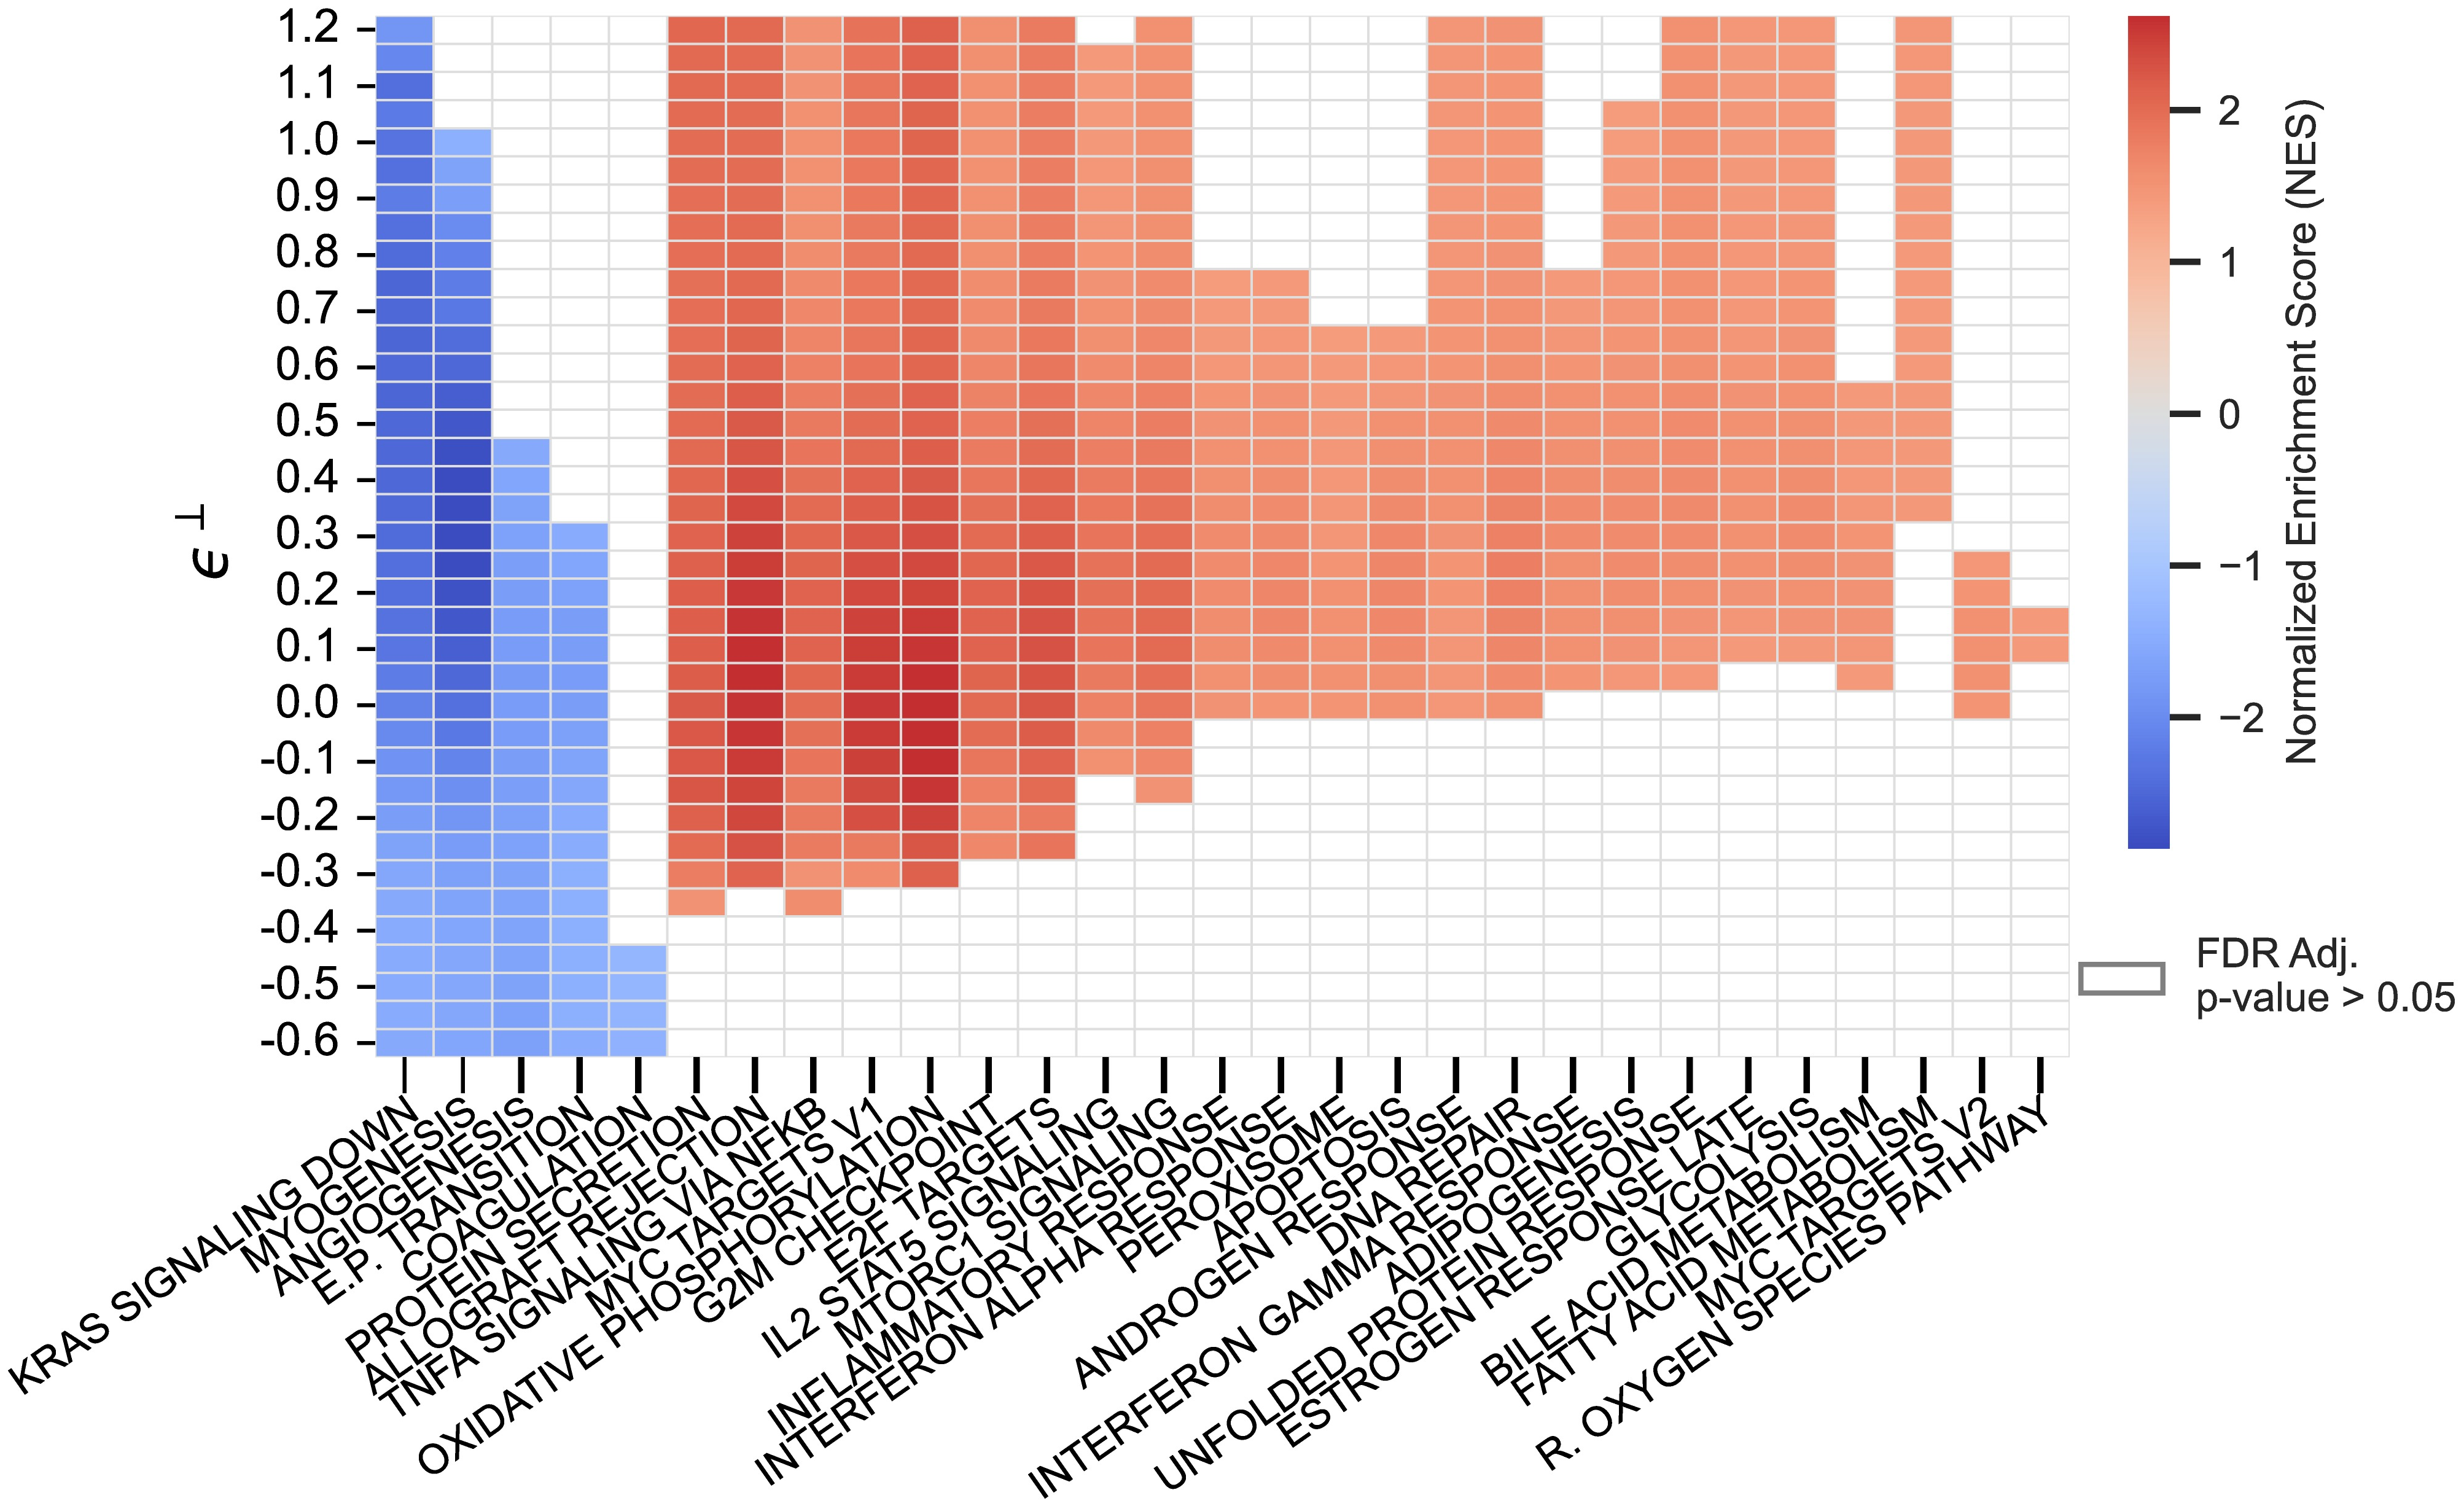
\includegraphics[scale=0.7]{/home/hh/data/output/thyroid_lfc_sens.png}
  \end{center}
\end{frame}

\begin{frame}
  \begin{center}
    Addressing the Problem of Inter-gene/microbe Correlations
  \end{center}
\end{frame}

\begin{frame}
  \frametitle{The Problem with Inter-gene/microbe correlations}

  \begin{center}
    \textbf{Are Random Gene Sets a Reasonable Method for Generating a Null Distribution?}
  \end{center}
  
  \begin{center}
    \begin{tabular}{| c | c | c | c | c | c | c | c | c | c |}
      \hline
      \makecell{Gene \\Name} & RB1 & IL2 & APP & AR & HTT & IL6 & B2M & RGN & CAT \\
      \hline
      Set \(S\) & X & & X & X & X & & & & \\
      \hline
      \hline
      Perm 1 & & X & X & & & & X & X & \\
      \hline
      Perm 2 & X & & & & & X & X & X & \\
      \hline
      \dots & & & & & & & & & \\
      \hline
      Perm Q & X & & & X & & & X & & X \\
      \hline
    \end{tabular}
  \end{center}
\end{frame}

\begin{frame}
  \frametitle{The Problem with Inter-gene/microbe Correlations}
  \begin{block}{Core Issue}
    Biologically related genes tend to be (positively) correlated, random genes tend to not be correlated. 
  \end{block}

   \begin{columns}
     \begin{column}{0.5\textwidth}
      \begin{center}
        \underline{Correlation Matrix: 5 Biologically}
        \underline{Related Genes}
        
        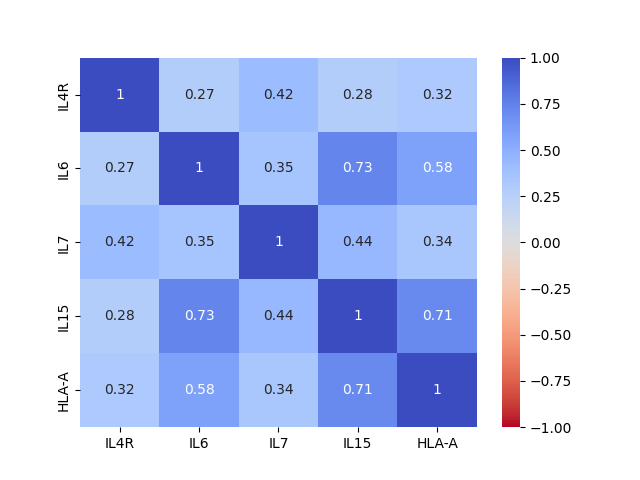
\includegraphics[scale=0.41]{/home/hh/data/output/corr_intf_gamma_res.png}
      \end{center}
    \end{column}
    \vrule{}
    \begin{column}{0.5\textwidth}  %%<--- here
      \begin{center}
        \underline{Correlation Matrix: 5 Random}
        \underline{Genes}
        
        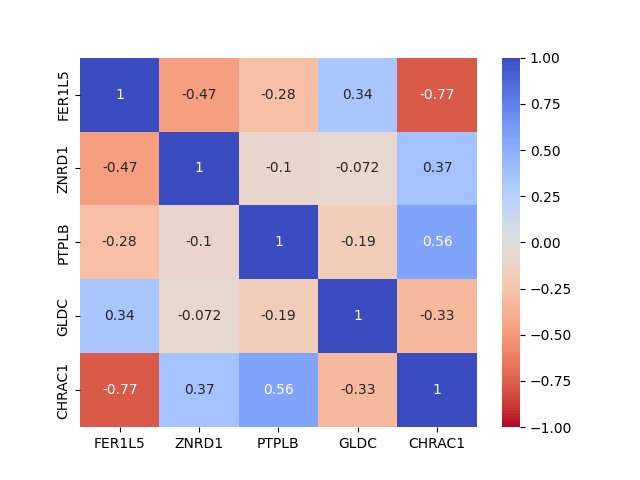
\includegraphics[scale=0.41]{/home/hh/data/output/corr_rand.png}
      \end{center}
    \end{column}
   \end{columns}
\end{frame}

\begin{frame}
  \frametitle{Correlations Inflate Flase Positives}
  Wu et al. considered a simulation with
  \begin{itemize}
    \item 10000 genes, \textbf{all with an LFC of 0}
    \item One gene set of 100 genes \textbf{with an average correlation of 0.05}
  \end{itemize}

  \pause

  Expected Results:
  \begin{itemize}
    \item No pathways/genes are enriched meaning the false positive rate should be around 5\%
  \end{itemize}

  \pause
    
  Actual Results:
  \begin{itemize}
    \item GSEA w/ gene label permutations had a false positive rate of up to 40\%!
  \end{itemize}
\end{frame}

\begin{frame}
  \frametitle{Two Methods for Addressing Inter-gene/microbe Correlations}

  \pause
  
  \begin{enumerate}
    \item GSEA with \textbf{sample label permutations}
\end{enumerate}
      \vspace{15px}
      \underline{GSEA with gene label permutations}
      \begin{align*}
        \hat{\theta} \implies \text{Permute Set } S \implies \text{Enrichment Score}
      \end{align*}

      \vspace{5px}
      \underline{GSEA with sample label permutations}
      \begin{align*}
        \log \hat{W} \implies \text{Permute Sample Labels } \implies \hat{\theta}^* \implies \text{Enrichment Score}
      \end{align*}

  
  
\end{frame}

\begin{frame}
  \frametitle{Two Methods for Addressing Inter-gene/microbe Correlations}
  \begin{enumerate}

    \setcounter{enumi}{1}
    
  \item CAMERA: Two-sample T-test \textbf{adjusted for correlation in \(S\)}

    \vspace{15px}

    Let:
    \begin{itemize}
      \item \(\theta_{\in S}, \theta_{\notin S}\) be LFCs of genes in/not-in set \(S\)
      \item \(\rho_S\) be the average correlation in gene expression for set \(S\) 
    \end{itemize}
   
  \begin{align*}
    T = \frac{\hat{\theta}_{\in S} - \hat{\theta}_{\notin S}}{s_p\sqrt{\frac{1+(n_1-1)\color{red}{\hat{\rho}_S}}{n_1} + \frac{1}{n_2}}}
  \end{align*}

  where

  \begin{align*}
    \color{red}{\hat{\rho}_S}\color{black}{ = f(\log \hat{W})}
  \end{align*}
  
  \end{enumerate}
\end{frame}

\begin{frame}
  \frametitle{Scale Sensitivity Analysis}

  \begin{itemize}
  \item Review: GSEA with Gene Label Permutations

    \vspace{10px}
    A function of LFCs
    \begin{align*}
      \phi_S = u(\theta)
    \end{align*}

    \vspace{10px}
    LFC Sensitivity Analysis:
    \begin{align*}
      \phi_S = u(\hat{\theta} + \pmb{1}\epsilon^\perp)
    \end{align*}
  \end{itemize}
  
\end{frame}

\begin{frame}
  \frametitle{Scale Sensitivity Analysis}

  \begin{itemize}
  \item GSEA with Sample Label Permutations / CAMERA

    A function of log absolute abundances:
    \begin{align*}
      \phi_S = u(\log W)
    \end{align*}

    \pause
    
    \begin{align*}
      \underbrace{\log W}_{\substack{D \times N \text{ Matrix} \\ \text{Abs Abundances}}} &= \underbrace{\log W^\parallel}_{\substack{D \times N \text{ Matrix} \\ \text{Compositions}}} + \underbrace{\log W^\perp}_{\substack{N \text{ length vector} \\ \text{ of scale}}} \\
    \end{align*}

    \pause

    \begin{align*}
      \underbrace{\begin{bmatrix}W^\perp_1 \\ \vdots \\ W^\perp_N \end{bmatrix}}_{\text{True Scale}} = \underbrace{\begin{bmatrix}\hat{W}^\perp_1 \\ \vdots \\ \hat{W}^\perp_N \end{bmatrix}}_{\text{Scale Assumption}} + \underbrace{\begin{bmatrix}\epsilon^\perp_1 \\ \vdots \\ \epsilon^\perp_N \end{bmatrix}}_{\substack{\text{Scale Assumption} \\ \text{Error}}}
    \end{align*}
  \end{itemize}
\end{frame}

\begin{frame}
  \frametitle{Scale Sensitivity Analysis}

  \begin{itemize}
  \item LFC Sensitivity Analysis
    \begin{align*}
      \phi_S &= u(\theta) \\
      \phi_S &= u(\hat{\theta}+\epsilon^\perp)
    \end{align*}
  \item Scale Sensitivity Analysis
     \begin{align*}
      \phi_S &= u(\log W) \\
      \phi_S &= u(\log \hat{W}+ [\epsilon^\perp_1,\dots,\epsilon^\perp_N]^T)
    \end{align*}
   
  \end{itemize}
\end{frame}


\begin{frame}[t]
  \frametitle{Two Scale Sensitivity Analyses}

    Scale Sensitivity Analysis \color{gray} (GSEA w/ sample label permutations and CAMERA) \color{black}
    \begin{align*}
      \phi_S &= u(\log W) \\
      \phi_S &= u(\log \hat{W} + \left[\epsilon^\perp_1,\dots,\epsilon^\perp_n\right])
    \end{align*}

   Here we consider 4500 gene sets in Healthy vs. Tumor breast tissue:
   \begin{columns}
     \begin{column}{0.5\textwidth}
      \begin{center}
        \underline{Constant Error}

        \begin{align*}
          \epsilon^\perp_i = \begin{cases}
            0 & \text{if } i \in \text{Healthy} \\
            \delta^\perp & \text{if } i \in \text{Tumor}
          \end{cases}
        \end{align*}
      \end{center}
    \end{column}
    \vrule{}
    \begin{column}{0.5\textwidth}  %%<--- here
      \vspace{5px}
      \begin{center}
        \underline{Sample-specific Error}
        
         \begin{align*}
          \epsilon^\perp_i \in [-\gamma^\perp,\gamma^\perp]
         \end{align*}
         \vspace{1px}
      \end{center}
    \end{column}
   \end{columns}
\end{frame}

\begin{frame}
  \frametitle{Two Scale Sensitivity Analyses}

     \begin{columns}
     \begin{column}{0.5\textwidth}
      \begin{center}
        \underline{Constant Error}

        \begin{align*}
          \epsilon^\perp_i = \begin{cases}
            0 & \text{if } i \in \text{Healthy} \\
            \delta^\perp & \text{if } i \in \text{Tumor}
          \end{cases}
        \end{align*}
      \end{center}
    \end{column}
    \vrule{}
    \begin{column}{0.5\textwidth}  %%<--- here
      \vspace{5px}
      \begin{center}
        \underline{Sample-specific Error}
        
         \begin{align*}
          \epsilon^\perp_i \in [-\gamma^\perp,\gamma^\perp]
         \end{align*}
         \vspace{1px}
      \end{center}
    \end{column}
   \end{columns}

     \begin{center}
       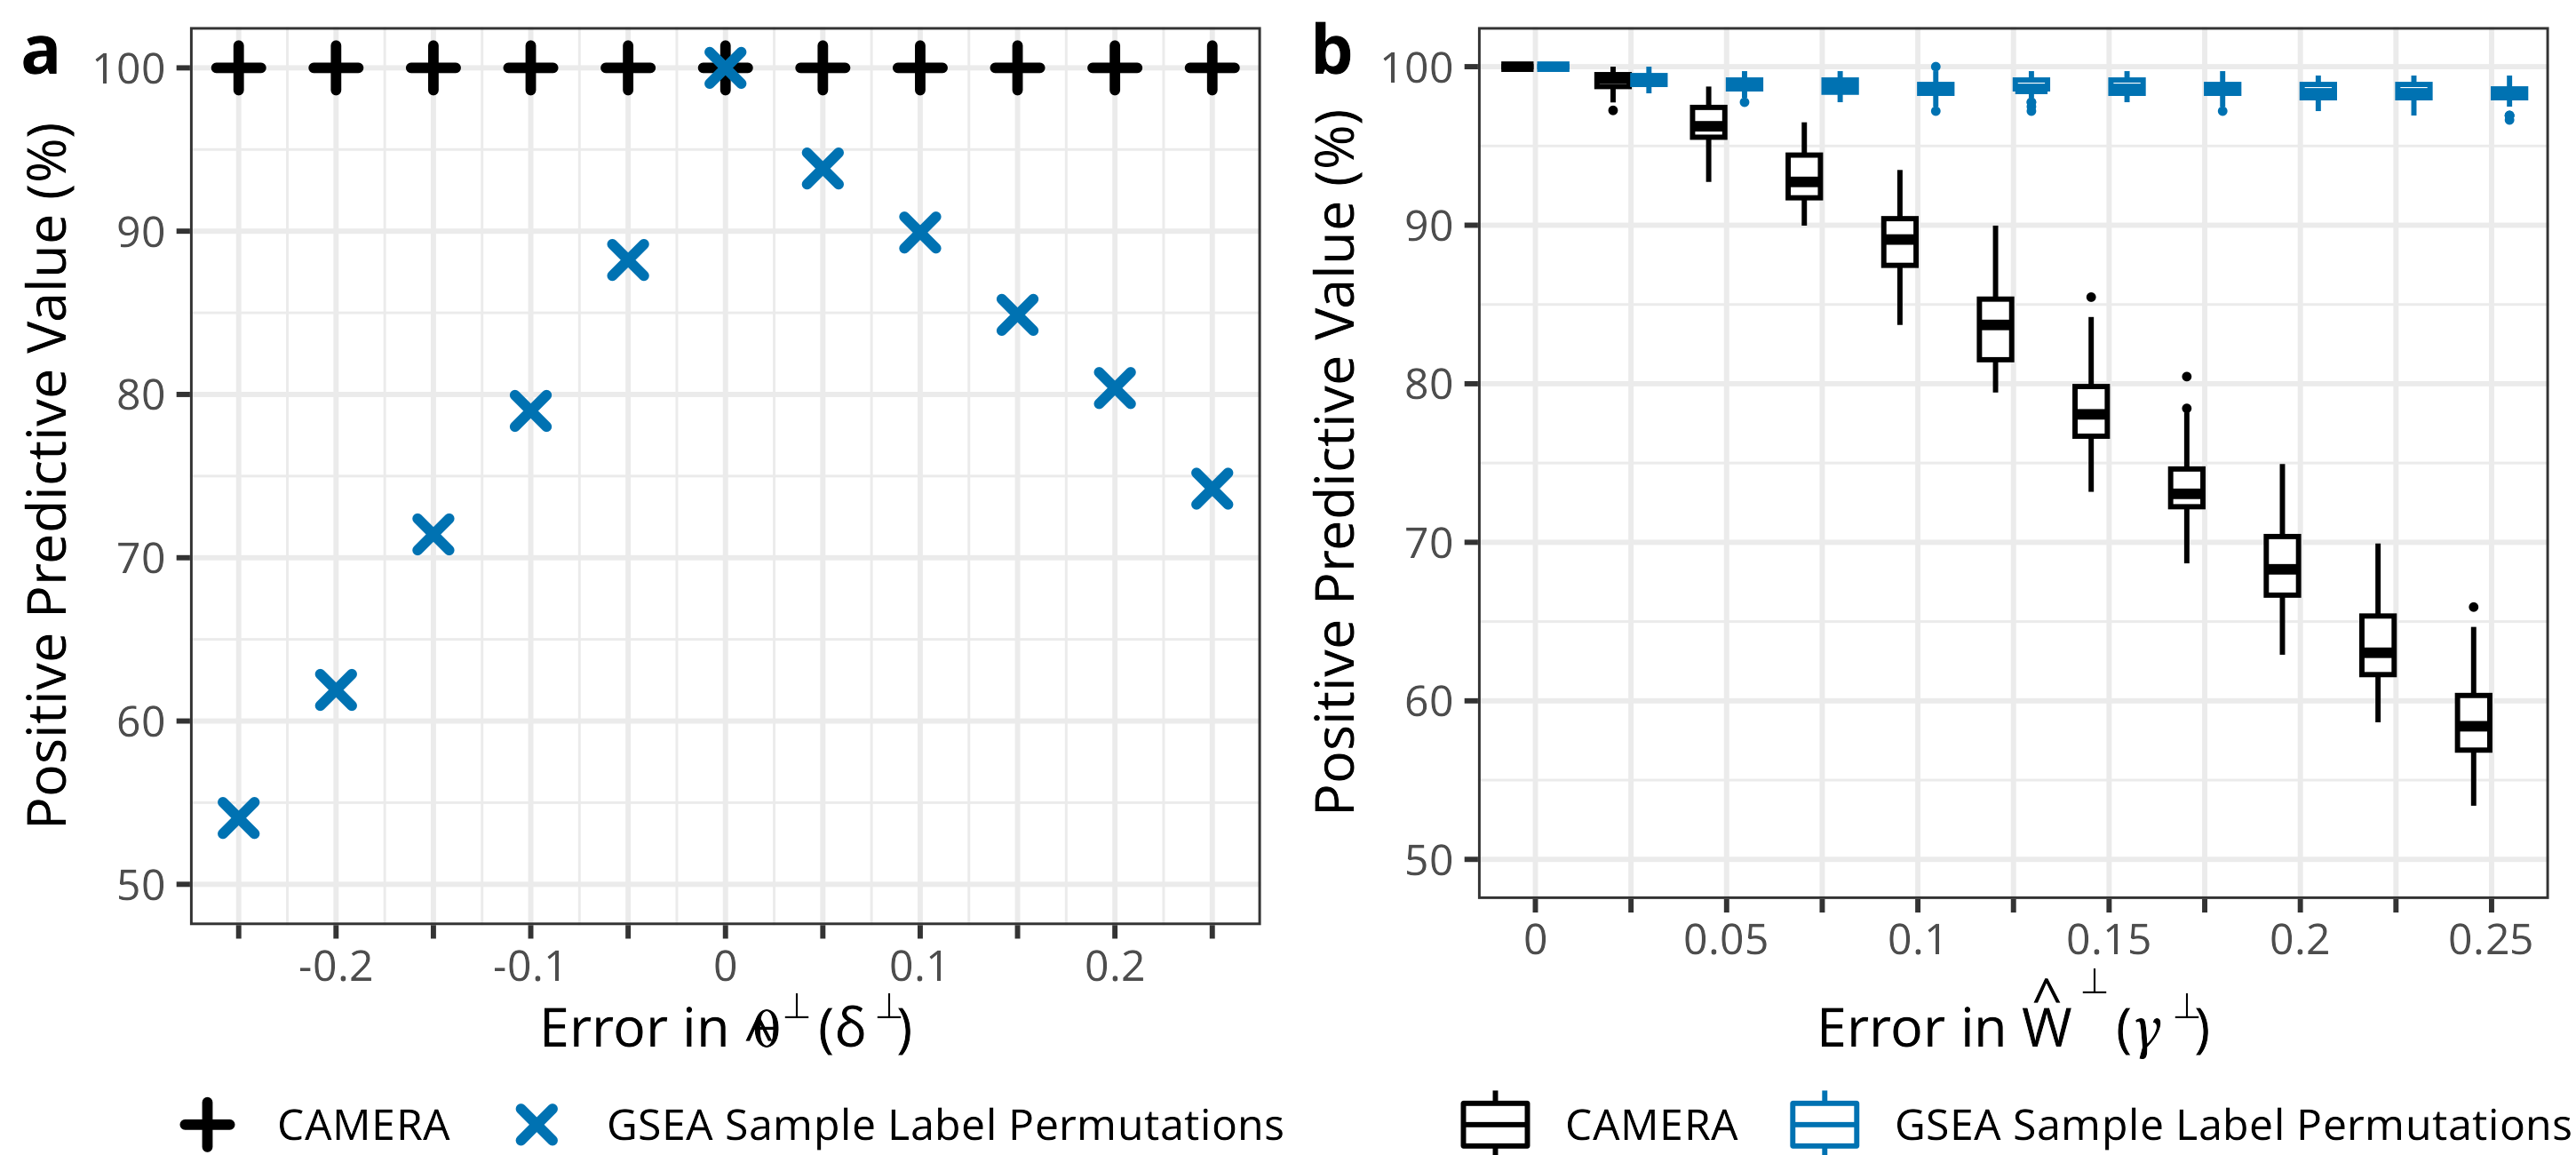
\includegraphics[scale=0.5]{/home/hh/data/output/Scale_Sensitivity_Analysis.png}
     \end{center}
\end{frame}

\begin{frame}
  \frametitle{References}

  \begin{enumerate}   
  \item \footnotesize{Gatti, et al. Heading down the wrong pathway: on the influence of correlation within gene sets. BMC Genomics. 2010 Oct 18;11:574. doi: 10.1186/1471-2164-11-574.}
  \item \footnotesize{McGovern, et al. Addressing erroneous scale assumptions in microbe and gene set enrichment analysis. PLoS Comput Biol. 2023 Nov 20;19(11):e1011659. doi: 10.1371/journal.pcbi.1011659.}
   \item \footnotesize{Subramanian, et al. Gene set enrichment analysis: a knowledge-based approach for interpreting genome-wide expression profiles. Proc Natl Acad Sci U S A. 2005 Oct 25;102(43):15545-50. doi: 10.1073/pnas.0506580102. Epub 2005 Sep 30.}
   \item \footnotesize{Wu, et al. Camera: a competitive gene set test accounting for inter-gene correlation. Nucleic Acids Res. 2012 Sep 1;40(17):e133. doi: 10.1093/nar/gks461. Epub 2012 May 25.}
     \item \footnotesize{Aran, et al. Comprehensive analysis of normal adjacent to tumor transcriptomes. Nat Commun. 2017 Oct 20;8(1):1077. doi: 10.1038/s41467-017-01027-z. PMID: 29057876; PMCID: PMC5651823.}
  \end{enumerate}
  
\end{frame}

\end{document}
